\documentclass[11pt]{beamer}
\usetheme{Warsaw}
\usepackage[frenchb]{babel}
\usepackage[T1]{fontenc}
\usepackage[utf8]{inputenc}
\usepackage{listings}
\usepackage{amsmath}
\usepackage{amsfonts}
\usepackage{amssymb}
\usepackage{forest}
\usepackage{xcolor}

\definecolor{folderbg}{RGB}{124,166,198}
\definecolor{folderborder}{RGB}{110,144,169}

\def\Size{4pt}
\tikzset{
  folder/.pic={
    \filldraw[draw=folderborder,top color=folderbg!50,bottom color=folderbg]
      (-1.05*\Size,0.2\Size+5pt) rectangle ++(.75*\Size,-0.2\Size-5pt);  
    \filldraw[draw=folderborder,top color=folderbg!50,bottom color=folderbg]
      (-1.15*\Size,-\Size) rectangle (1.15*\Size,\Size);
  }
}

\lstset{language=C++,
	basicstyle=\tiny\ttfamily,
	keywordstyle=\color{blue}\ttfamily,
	stringstyle=\color{red}\ttfamily,
	commentstyle=\color{green}\ttfamily,
	morecomment=[l][\color{magenta}]{\#},
	breaklines=true,
	breakatwhitespace=true
}

\author{Lazare Lucas - Pinard Maxime}
\title{Présentation TZ20}
%\setbeamercovered{transparent} 
%\setbeamertemplate{navigation symbols}{} 
%\logo{} 
\institute{UTBM} 
\date{\today} 
\subject{TZ20} 
\begin{document}

\begin{frame}
	\titlepage{}
\end{frame}

\begin{frame}
	\tableofcontents{}
\end{frame}

\section{Objectifs}

	\begin{frame}
		\frametitle{Objectifs}
		\begin{itemize}
			\item{} Restriction d'accès
			\item{} Dossier privé et publique
			\item{} Affichage fonction \textit{ls}
			\item{} Suppression des fichier (24h)
			\item{} Logs de connexion
			\item{} Changement de mot de passe
			\item{} Descriptions de fichiers
			\item{} Création de nouveaux comptes
			\item{} Configuration du serveur
		\end{itemize}
	\end{frame}

\section{Problèmes}

	\begin{frame}
		\frametitle{Problèmes}
		\begin{itemize}
			\item{} Communication client - serveur
			\item{} Interprétation des commandes
			\item{} Gerer les restrictions d'accès
			\item{} Récupérer la liste des dossiers et fichiers présents dans un dossier
			\item{} Stocker des informations à propos des dossiers et fichiers uploadés
			\item{} Afficher des informations de façon ergonomique/lisible
			\item{} Envoyer des mails via un programme
			\item{} Créer, gérer et utiliser la configuration du serveur
			\item{} Permettre au client de télécharger / uploader un dossier complet
		\end{itemize}
	\end{frame}

\section{Solutions}
	\subsection{Architecture}

		\begin{frame}
			\frametitle{Architecture}
			%\framesubtitle{avec un exemple de sous-titre}
			\begin{forest}
			  for tree={
			    font=\ttfamily,
			    grow'=0,
			    child anchor=west,
			    parent anchor=south,
			    anchor=west,
			    calign=first,
			    inner xsep=7pt,
			    edge path={
			      \noexpand\path [draw, \forestoption{edge}]
			      (!u.south west) +(7.5pt,0) |- (.child anchor) pic {folder} \forestoption{edge label};
			    },
			    before typesetting nodes={
			      if n=1
			        {insert before={[,phantom]}}
			        {}
			    },
			    fit=band,
			    before computing xy={l=15pt},
			  }  
			[server execution folder
			  [Downloading\_Threads
			  ]
			  [FilesData
			  ]
			  [IPList
			  ]
			  [Public
			  ]
			  [Private
			  ]
			  [ToConf
			  ]
			  [UsersData
			  ]
			]
			\end{forest}
		\end{frame}

	\subsection{Interface}

		\begin{frame}
			\frametitle{Interface}
			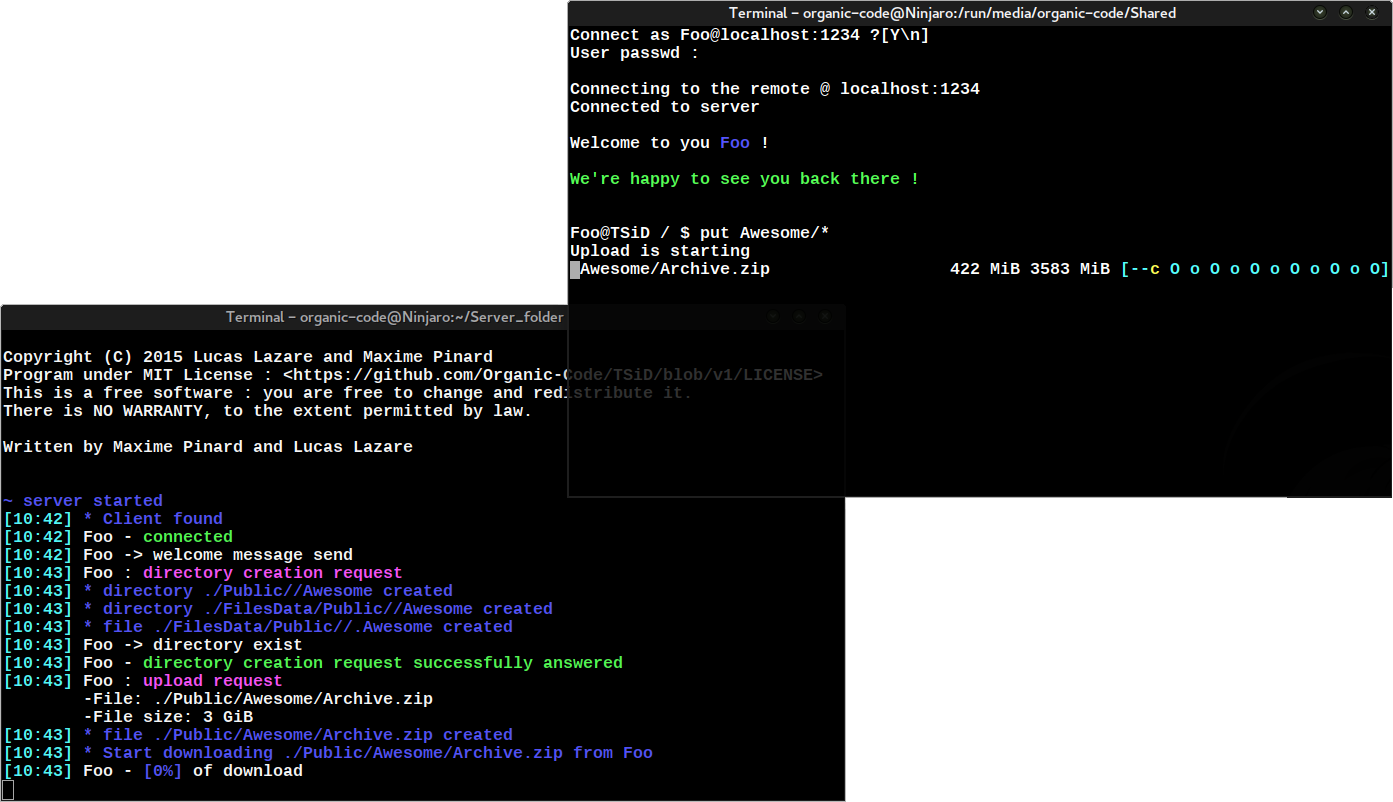
\includegraphics[width=\linewidth]{interface}
		\end{frame}
\begin{frame}[fragile]
\frametitle{code}
\begin{lstlisting}
//code
\end{lstlisting}
\end{frame}
\end{document}
